%%%%%%%%%%%%%%%%%%%%%%%%%%%%%%%%%%%%%%%%%%%%%%%%%%%%%%%%%%%%%%%%%%%%%%%%%%%%%%%
\chapter{Zero absoluto}
\label{Chap:ExpZeroAbsoluto}
%%%%%%%%%%%%%%%%%%%%%%%%%%%%%%%%%%%%%%%%%%%%%%%%%%%%%%%%%%%%%%%%%%%%%%%%%%%%%%%

\begin{fullwidth}\it
	Realizaremos um experimento em que verificaremos a pressão exercida por uma quantidade de gás com volume constante em função de sua temperatura. Através desses dados, determinaremos a temperatura para a qual teríamos uma pressão nula -- tal temperatura é o que denominamos como Zero Absoluto --. Utilizaremos os seguintes conceitos/técnicas de análise de dados: medidas, algarismos significativos, gráficos, software para elaboração de gráficos, erros de escala e propagados, equação geral para o erro propagado, regressão linear, linearização, erros dos coeficientes $A$ e $B$, e planílhas para cálculo dos coeficientes $A$ e $B$ com erros.
\end{fullwidth}

%%%%%%%%%%%%%%%%%%%%%%%%%%%%%%%%%%%%%%%%%%%%%%%%%%%%%%%%%%%%%%%%%%%%%%%%%%%%%%%
\section{Termômetros}
%%%%%%%%%%%%%%%%%%%%%%%%%%%%%%%%%%%%%%%%%%%%%%%%%%%%%%%%%%%%%%%%%%%%%%%%%%%%%%%

Um método simples para verificar a temperatura é utilizar alguma propriedade de um material que varie com a temperatura como indicador de leitura. Alguns termômetros usam mercúrio, outros usam álcool. Em ambos os casos, a propriedade que varia com a temperatura é o volume: o líquido de um reservatório se dilata e invade um tubo fino, onde a altura da coluna pode ser lida através de uma escala.

Outras propriedades podem ser utilizadas para verificar a temperatura, dentre elas a tensão entre uma junção bi-metálica, a resistência elétrica de um material, o comprimento de uma fita metálica longa, a pressão de um volume confinado de um gás, etc. 

Em todos esses casos, é necessário se utilizar dois pontos para calibrar o termômetro com valores arbitrários de temperatura. A escala Celsius, por exemplo, utiliza a temperatura de fusão do gelo para zero graus e a temperatura de ebulição da água para 100 graus. No caso de um termômetro de mercúrio, por exemplo, podemos verificar a altura da coluna para a temperatura de fusão do gelo, realizando uma marca (na escala Celsius, zero). Marcamos também a altura da coluna para a temperatura de ebulição da água (na escala Celsius, \np[\tcdegree]{100}). Dividimos então o intervalo entre essas duas marcas em um número de divisões menores (na escala Celsius, são 100 divisões). Podemos então verificar qualquer temperatura intermediária utilizando uma leitura da coluna de mercúrio. Podemos inclusive extrapolar as leituras para valores de temperatura maiores e menores que os extremos definidos pela temperatura de fusão do gelo e de ebulição da água, bastando para isso manter o tamanho da divisão igual às divisões intermediárias.

A confiabilidade das medidas de temperatura obtidas através de um termômetro está diretamente ligada à linearidade da propriedade observada com a variação da temperatura. Para faixas de temperatura relativamente pequenas, isso pode não ser um problema, mas se desejarmos realizar medições para ampla faixa de valores comportamentos não-lineares podem ter efeito significativo. Além disso, se -- por exemplo -- desejarmos utilizar uma medida de temperatura extremamente elevada, não podemos utilizar um termômetro devido ao risco de danificá-lo. Portanto, é importante escolher um material e uma propriedade adequados à medida em questão.

%%%%%%%%%%%%%%%%%%%%%%%%%%%%%%%%%%%%%%%%%%%%%%%%%%
\subsection{Termômetros de gás a volume constante}
%%%%%%%%%%%%%%%%%%%%%%%%%%%%%%%%%%%%%%%%%%%%%%%%%%

Uma propriedade que pode ser utilizada para realizar uma medida confiável da temperatura é a pressão de um gás mantido em um volume constante. Segundo a equação dos gases ideais, a pressão varia com a temperatura de acordo com
\begin{equation}
	PV = nRT,
\end{equation}
%
onde $R$ é a constante dos gases, $n$ é o número de moles de partículas do gás, $V$ é o volume ocupado pelo gás e $T$ é a temperatura na escala Kelvin (discutida adiante). Dessa equação, podemos escrever
\begin{equation}\label{Eq:PvsT}
	P = \frac{nR}{V} T.
\end{equation}

\begin{marginfigure}
\centering
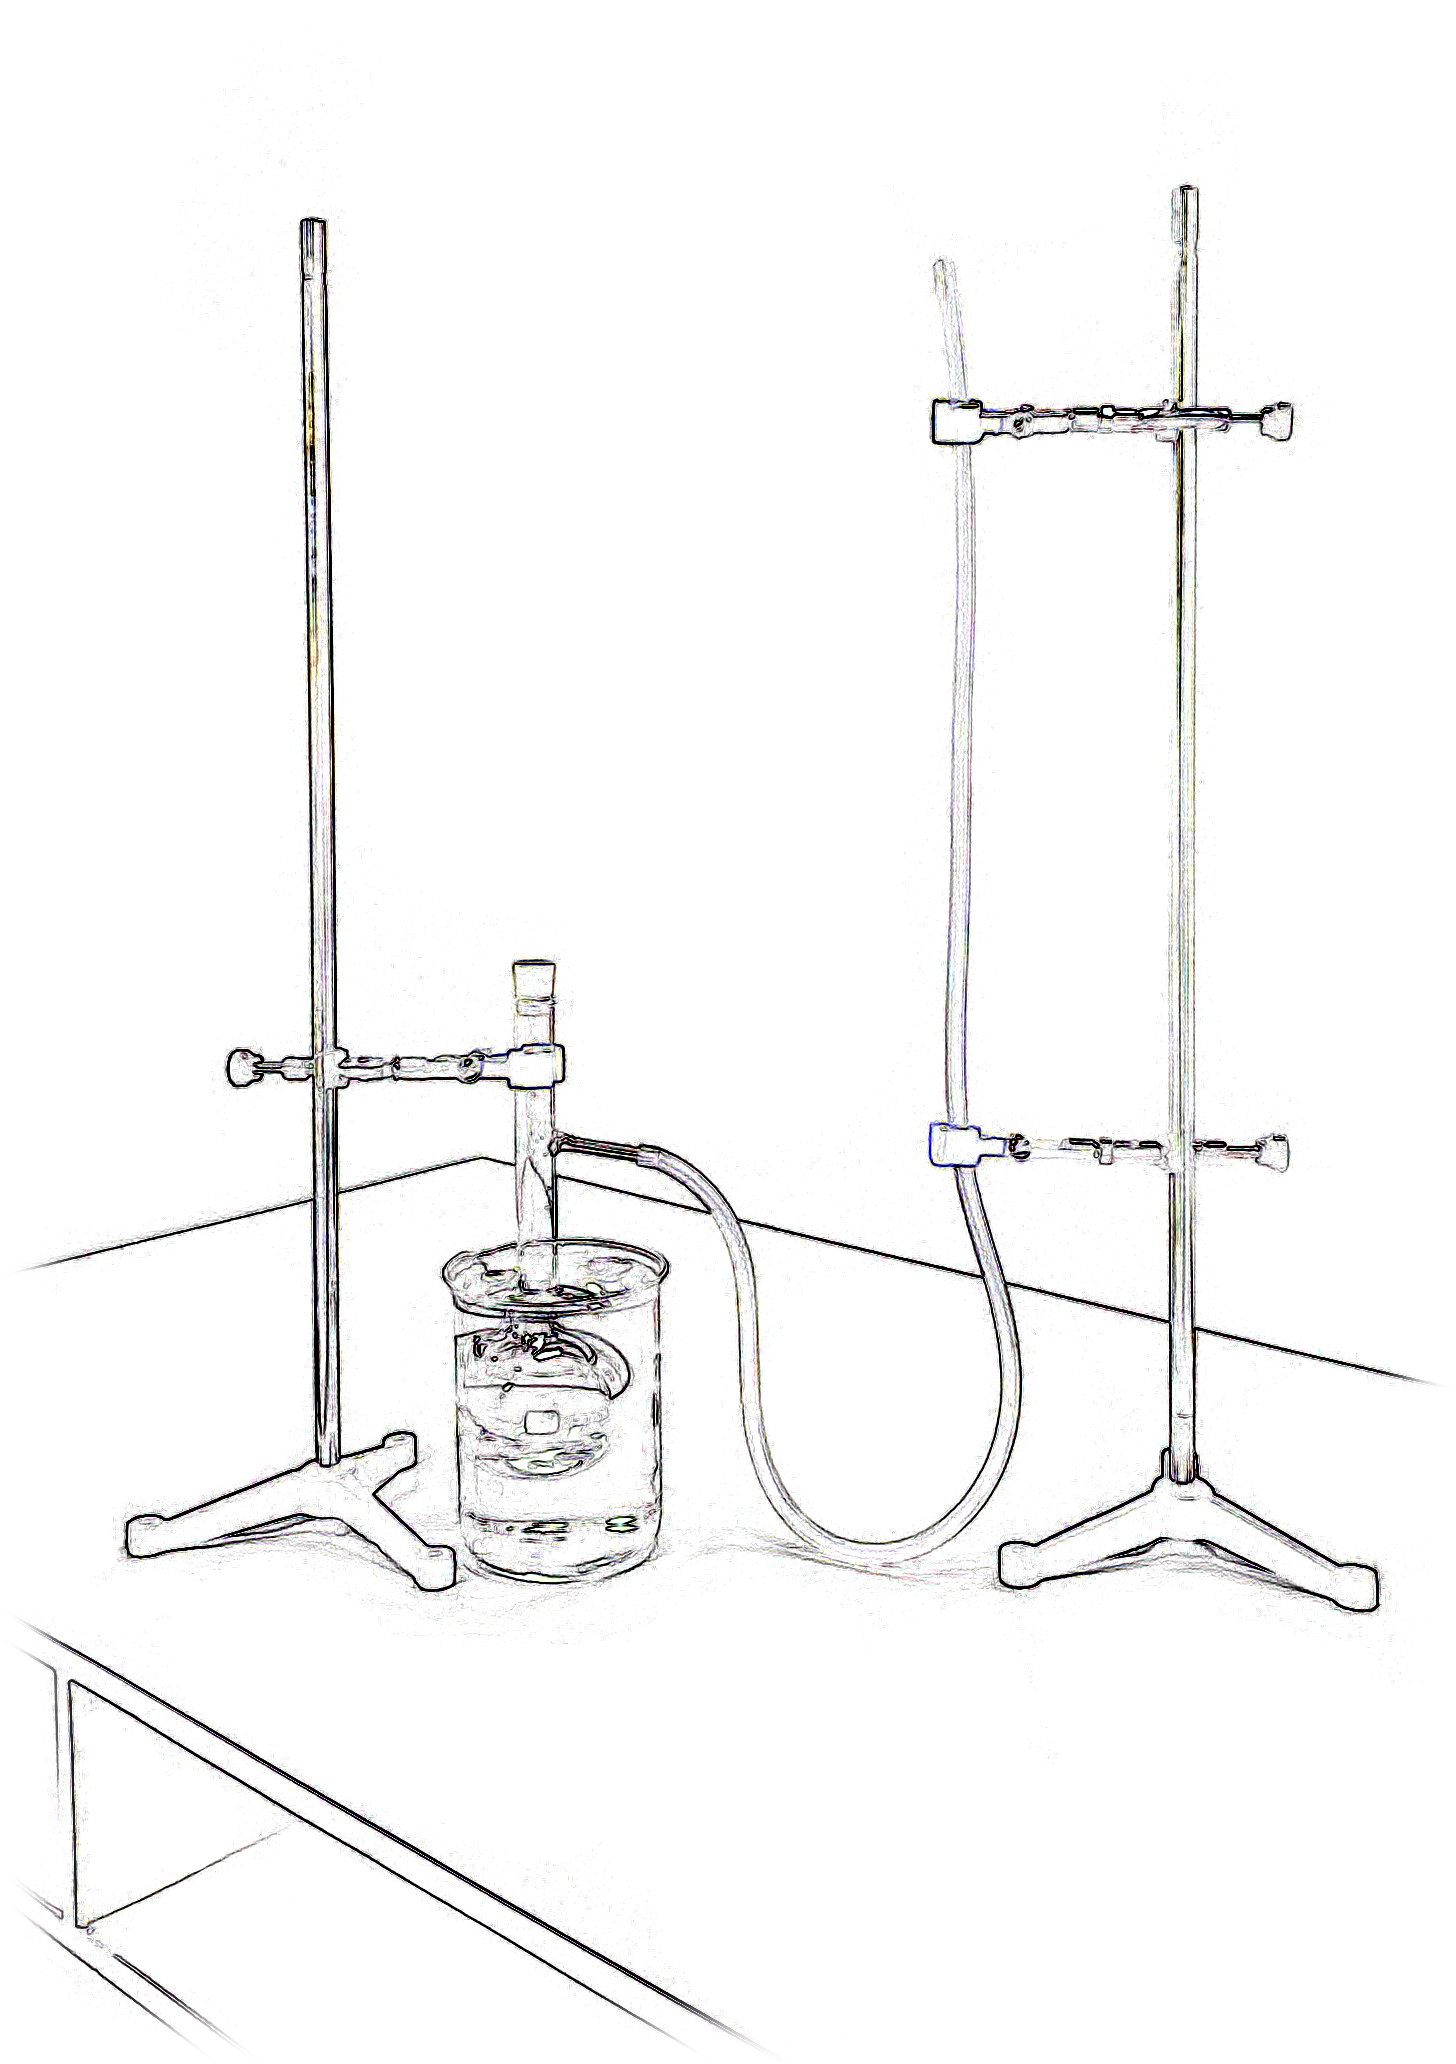
\includegraphics[width=\textwidth]{Ilustrations/Term_gas.png}
\caption{Termômetro de gás a volume constante.}
\label{Fig:TermometroGas}
\end{marginfigure}
Para um gás mantido a um volume $V$ constante em um reservatório, podemos afirmar que o número de moles $n$ se mantém constante. Temos então uma relação de proporcionalidade entre a pressão do gás e a temperatura a que ele se encontra. Um dispositivo que utiliza essa propriedade para realizar medidas é denominado \textbf{termômetro de gás a volume constante}. A Figura~\ref{Fig:TermometroGas} mostra um desenho esquemático desse tipo de dispositivo.

Neste termômetro, pressão do gás será determinada pela pressão exercida pela coluna de líquido (pois ela equilibra a pressão do recipiente com o gás), sendo que seu valor será dado por
\begin{equation}
	P = P_0 + \rho g h,
\end{equation}
%
onde $P_0$ é a pressão atmosférica, $\rho$ é a densidade da água, $g$ é a aceleração da gravidade e $h$ é a altura da coluna de líquido. A altura $h$ deve ser medida na extremidade aberta do tubo, a partir do nível da coluna de água na extremidade que está ligada ao recipiente com o gás.

Para um gás real, a relação entre a pressão e a temperatura depende do tipo de gás utilizado. Porém, se o gás estiver a baixa pressão, ou seja, estiver \emph{rarefeito}, e a temperatura a ser medida for maior que aquela em que o gás se torna um líquido, podemos utilizar qualquer gás para realizar medidas de temperatura. A diferença entre diversos gases será a inclinação da reta, porém as relações serão sempre lineares.

%%%%%%%%%%%%%%%%%%%%%%%%%%
\subsection{Zero absoluto}
%%%%%%%%%%%%%%%%%%%%%%%%%%

Para qualquer gás utilizado no termômetro, a medida que a temperatura diminui, a pressão do gás também diminui. Essa relação deve ter um valor para o qual q pressão exercida pelo gás é nula, correspondendo a uma temperatura mínima ou um \textbf{zero absoluto} para a escala de temperatura. Apesar de a inclinação das retas de $P \times T$ serem diferentes para gases diferentes, o valor para o qual a pressão é zero é o mesmo para qualquer gás, sendo que tal valor corresponde a $-\np[\tcdegree C]{273,15}$. Podemos então utilizar o valor do zero absoluto para definir uma escala de temperaturas -- a escala Kelvin -- em que a menor temperatura possível seja zero, correspondendo ao zero absoluto, e na qual a temperatura de fusão do gelo seja \np[K]{273,15}, sendo que a relação entre tal escala e a escala Celsius será dada por
\begin{equation}\label{Eq:RelKC}
	T_C = T - \np{273.15}.
\end{equation}

De acordo com a interpretação cinética para os gases, a pressão exercida pelo gás está relacionada à energia cinética das partículas que o compõe: a pressão é exercida nas paredes de um recipiente pelas colisões sucessivas das partículas que compõe o gás. Ao se atingir o zero absoluto, a pressão e a energia cinética das partículas serão nulas\footnote{Se não há pressão, isso só pode ser explicado pela ausência de colisões entre as partículas do gás e as paredes do recipiente, o que implica que as partículas estão em repouso em relação ao recipiente e que --~consequentemente~-- suas energias cinéticas são nulas.}, o que correspoderia classicamente a todas as partículas do gás repousarem no fundo do recipiente que as contém.

%%%%%%%%%%%%%%%%%%%%%%%%%%%%%%%%%%%%%%%%%%%%%%%%%%%%%%%%%%%%%%%%%%%%%%%%%%%%%%%
\section{Experimento}
%%%%%%%%%%%%%%%%%%%%%%%%%%%%%%%%%%%%%%%%%%%%%%%%%%%%%%%%%%%%%%%%%%%%%%%%%%%%%%%

%%%%%%%%%%%%%%%%%%%%%%
\subsection{Objetivos}
%%%%%%%%%%%%%%%%%%%%%%

\begin{itemize}
	\item Verificar que a relação entre a pressão de um gás com a temperatura é linear.
	\item Calcular o valor do zero absoluto na escala Celsius.
\end{itemize}

%%%%%%%%%%%%%%%%%%%%%%%%%%%%%%%%%%%%%%%%%%%%%%%%%%%%%%%%%%%%%%%%%%%%%%%%%%%%%%%
\section{Material Necessário}
%%%%%%%%%%%%%%%%%%%%%%%%%%%%%%%%%%%%%%%%%%%%%%%%%%%%%%%%%%%%%%%%%%%%%%%%%%%%%%%

\begin{multicols}{2}
\begin{itemize}
	\item Becker;
	\item Balão volumétrico com saída lateral;
	\item Rolha;
	\item Suporte vertical com garras;
	\item Termômetro;
	\item Tubo flexível transparente longo;
	\item Réguas e trenas;
	\item Bastão de vidro;
	\item Recipiente com água;
	\item Tela de amianto e suporte para a tela;
	\item Lamparina e fósforos;
	\item Flanela.
\end{itemize}
\end{multicols}

\begin{figure}[!h]
\centering
\forceversofloat
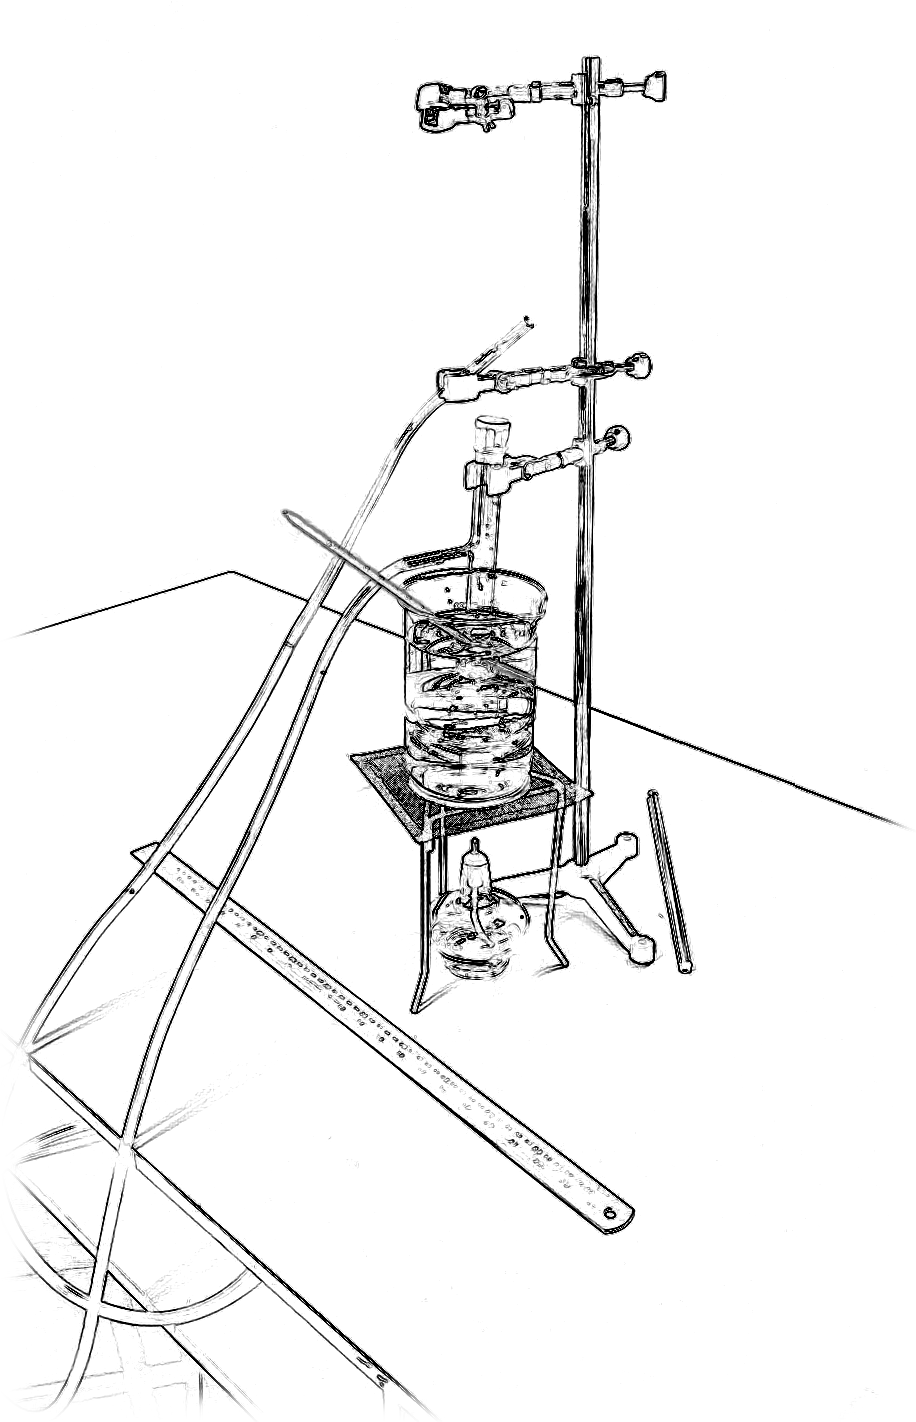
\includegraphics[width=0.7\textwidth]{Ilustrations/AparatoZeroAbs.png}
\caption{Aparato para a verificação do zero absoluto.}
\end{figure}
%%%%%%%%%%%%%%%%%%%%%%%%%%%%%%%%%%%%%%%%%%%%%%%%%%%%%%%%%%%%%%%%%%%%%%%%%%%%%%%
\section{Procedimento Experimental}
%%%%%%%%%%%%%%%%%%%%%%%%%%%%%%%%%%%%%%%%%%%%%%%%%%%%%%%%%%%%%%%%%%%%%%%%%%%%%%%

\begin{enumerate}
\item Disponha a tela de amianto sobre o suporte e coloque o becker sobre ela;
\item Disponha o suporte vertical próximo ao becker. Afixe nele uma garra e a utilize para segurar o balão de destilação. A parte arredondada do balão deve ficar disposta dentro do becker, porém sem tocar o fundo;
\item Adicione água ao tubo de forma que ele fique sem bolhas e com água até aproximadamente \np[cm]{20} de cada extremidade;
\item Prenda o tubo ao suporte com o auxílio de garras de forma que uma das extremidades possa ser presa ao balão e que a outra fique à mesma altura que a primeira (a parte restante do tubo deve ficar abaixo da mesa, no chão);
\item Prenda uma das extremidades do tubo à saída lateral do balão volumétrico;
\item Feche a saída do balão com a rolha;
\item Verifique a pressão atmosférica $P_0$ e a anote na Tabela~\ref{Tab:Dados};
\item Se houver variação na altura da coluna d'água ao fechar a rolha, meça a distância \textbf{vertical} entre os dois meniscos, calcule a pressão associada a tal coluna e a adicione à pressão $P_0$ na Tabela~\ref{Tab:Dados}.
\item Adicione água ao becker até cobrir a parte arredondada do balão e parte do gargalo;
\item Verifique a temperatura da água com o termômetro e anote na Tabela~\ref{Tab:Dados}. Também verifique a altura da coluna d'água na extremidade ligada ao balão e a marque no tubo.
\item Disponha a lamparina abaixo da tela de amianto e a acenda.
\item Agite a água constantemente para que ela tenha uma temperatura homogênea; 
\item Assim que a temperatura\footnote{Meça na altura da metade do balão, nem muito acima, nem muito abaixo. Para evitar inomogeneidades na temperatura, o ideal é apagar a lamparina e agitar a água por alguns segundos, anotando a temperatura atingida no equilíbrio térmico.} aumentar \np[\tcdegree]{5} , levante a extremidade livre do tudo de forma que o nível na extremidade ligada ao balão volte ao nível original. Verifique o valor da temperatura e a altura da coluna d'água (diferença de distância vertical entre o nível da extremidade aberta e o nível da extremidade ligada ao balão) e anote na Tabela~\ref{Tab:Dados}.
\item Aguarde até que o nivel volte a diminuir \np[cm]{2,00} ou \np[cm]{3,00}, reajuste o nível e anote os novos valores de altura da coluna e de temperatura correspondente na Tabela~\ref{Tab:Dados}. Repita esse processo de forma a obter o maior número de dados experimentais possível.
\end{enumerate}

%%%%%%%%%%%%%%%%%%%%%%%%%%%%%%%%%%%%%%%%%%%%%%%%%%%%%%%%%%%%%%%%%%%%%%%%%%%%%%%
%%%%%%%%%%%%%%%%%%%%%%%%%%%%%%%%%%%%%%%%%%%%%%%%%%%%%%%%%%%%%%%%%%%%%%%%%%%%%%%
%%%%%%%%%%%%%%%%%%%%%%%%%%%%%%%%%%%%%%%%%%%%%%%%%%%%%%%%%%%%%%%%%%%%%%%%%%%%%%%
%%%%%%%%%%%%%%%%%%%%%%%%%%%%%%%%%%%%%%%%%%%%%%%%%%%%%%%%%%%%%%%%%%%%%%%%%%%%%%%
\cleardoublepage

\noindent{}{\huge\textit{Zero absoluto}}

\vspace{15mm}

\begin{fullwidth}
\noindent{}\makebox[0.6\linewidth]{Turma:\enspace\hrulefill}\makebox[0.4\textwidth]{  Data:\enspace\hrulefill}
\vspace{5mm}

\noindent{}\makebox[0.6\linewidth]{Aluno(a):\enspace\hrulefill}\makebox[0.4\textwidth]{  Matrícula:\enspace\hrulefill}

\noindent{}\makebox[0.6\linewidth]{Aluno(a):\enspace\hrulefill}\makebox[0.4\textwidth]{  Matrícula:\enspace\hrulefill}

\noindent{}\makebox[0.6\linewidth]{Aluno(a):\enspace\hrulefill}\makebox[0.4\textwidth]{  Matrícula:\enspace\hrulefill}

\noindent{}\makebox[0.6\linewidth]{Aluno(a):\enspace\hrulefill}\makebox[0.4\textwidth]{  Matrícula:\enspace\hrulefill}

\noindent{}\makebox[0.6\linewidth]{Aluno(a):\enspace\hrulefill}\makebox[0.4\textwidth]{  Matrícula:\enspace\hrulefill}
\end{fullwidth}

\vspace{5mm}

%%%%%%%%%%%%%%%%%%%%%%%%%%%%%%%%%%%%%%%%%%%%%%%%%%%%%%%%%%%%%%%%%%%%%%%%%%%%%%%
\section{Questionário}
%%%%%%%%%%%%%%%%%%%%%%%%%%%%%%%%%%%%%%%%%%%%%%%%%%%%%%%%%%%%%%%%%%%%%%%%%%%%%%%

\begin{question}[type={exam}]{1}
Apresente os resultados de maneira clara e organizada. Mostre os cálculos requisitados de maneira clara e sucinta, evidenciando o raciocínio desenvolvido.
\end{question}

\begin{question}[type={exam}]{1}
Liste os equipamentos utilizados descrevendo o tipo do equipamento, sua resolução, e qual é o seu erro de escala.
\end{question}

\begin{question}[type={exam}]{2}
Preencha as tabelas com o número adequado de algarismos significativos, unidades, e erros de escala apropriados. 
\end{question}

\begin{question}[type={exam}]{2}
Elabore um gráfico de $P \times T$ para os dados da Tabela~\ref{Tab:Dados}. Calcule a reta que melhor representa os dados experimentais utilizando o método dos mínimos quadrados e a adicione ao gráfico.
\end{question}

\begin{question}[type={exam}]{2}
Mostre que, a partir da equação para a pressão em função a temperatura, podemos escrever a relação
\begin{equation}\label{Eq:EqRazaoABZeroAbs}
	T_0 = -\frac{A}{B}.
\end{equation}
%
Utilizando essa equação e os coeficientes para a regressão linear obtidos na questão anterior, calcule o valor de temperatura para o qual a pressão será zero. Verifique o erro percentual entre tal valor de temperatura e o valor de referência $T_0^{\textrm{ref}} = -\np[\tcdegree C]{273,15}$ através da expressão
\begin{equation}
	E_{\%} = \left|\frac{x-x_{\textrm{ref}}}{x_{\textrm{ref}}}\right| \times 100.
\end{equation}
\end{question}

\begin{question}[type={exam}]{3}
Calcule os erros associados aos coeficientes $A$ e $B$ da regressão linear e --~a partir dos coeficientes, dos erros a eles associados, e da Equação~\ref{Eq:EqRazaoABZeroAbs}~--  calcule o erro associado a $T_0$.
\end{question}

\begin{question}[type={exam}]{2}
Através dos resultados obtidos nas questões anteriores, discuta quais objetivos foram atingidos com sucesso, justificando suas conclusões. Se algum objetivo não foi atingido, discuta quais são os possíveis motivos do fracasso e que medidas podem ser tomadas para que eles sejam alcançados.
\end{question}

%%%%%%%%%%%%%%%%%%%%%%%%%%%%%%%%%%%%%%%%%%%%%%%%%%%%%%%%%%%%%%%%%%%%%%%%%%%%%%%
\section{Tabelas}
%%%%%%%%%%%%%%%%%%%%%%%%%%%%%%%%%%%%%%%%%%%%%%%%%%%%%%%%%%%%%%%%%%%%%%%%%%%%%%%

\begin{table*}[!htb]
\caption{Dados para a altura da coluna de água em função da temperatura.}
\label{Tab:Dados}
	\begin{center}
		\begin{tabular}{cp{45mm}p{45mm}p{45mm}c}
		\toprule
		&\multicolumn{2}{l}{\textbf{Constantes}}\\
		\cmidrule{2-3}
		& \cellcolor[gray]{0.89} $P_0$ &\cellcolor[gray]{0.92} \\
		& \cellcolor[gray]{0.95} $\rho$ & \cellcolor[gray]{0.97}\\
		\cmidrule{2-3}
		\\
		&\multicolumn{2}{l}{\textbf{Dados para a altura da coluna}} \\
		\cmidrule{2-4}
		& $T$ & $h$ & $P$ & \\
		\cmidrule{2-4}
		& \cellcolor[gray]{0.89} & \cellcolor[gray]{0.92} & \cellcolor[gray]{0.89} \\
		& \cellcolor[gray]{0.95} & \cellcolor[gray]{0.97} & \cellcolor[gray]{0.95} \\
		& \cellcolor[gray]{0.89} & \cellcolor[gray]{0.92} & \cellcolor[gray]{0.89} \\
		& \cellcolor[gray]{0.95} & \cellcolor[gray]{0.97} & \cellcolor[gray]{0.95} \\
		& \cellcolor[gray]{0.89} & \cellcolor[gray]{0.92} & \cellcolor[gray]{0.89} \\
		& \cellcolor[gray]{0.95} & \cellcolor[gray]{0.97} & \cellcolor[gray]{0.95} \\
		& \cellcolor[gray]{0.89} & \cellcolor[gray]{0.92} & \cellcolor[gray]{0.89} \\
		& \cellcolor[gray]{0.95} & \cellcolor[gray]{0.97} & \cellcolor[gray]{0.95} \\
		& \cellcolor[gray]{0.89} & \cellcolor[gray]{0.92} & \cellcolor[gray]{0.89} \\
		& \cellcolor[gray]{0.95} & \cellcolor[gray]{0.97} & \cellcolor[gray]{0.95} \\
		\cmidrule{2-4}
		\bottomrule
		\end{tabular}
	\end{center}
\end{table*}

